\subsection{Machine architecture and number systems}

\begin{definition}[von Neumann architecture]
	The \emph{von Neumann architecture} is a design architecture for a computer
	which consists of
	\begin{enumerate}
		\item a processing nuit;
		\item a control unit;
		\item memory that stores data and instructions;
		\item external mass storage; and
		\item input and output mechanisms.
	\end{enumerate}
	There is a data bus and an instruction betweeen the memory unit and
	processing unit.
\end{definition}

The \emph{Little Man Computer} (LMC) is a simple model of a von-Neumann
computer consisting of mailboxs, a calculator, a program counter, and a
input and output tray.

A LMC instruction is three digits. The first digit represents the
\emph{opcode} and the second and third digit is the \emph{operand}.
The following are opcodes in LMC.
\begin{enumerate}
	\item \emph{LDA}, load data from mailbox into the calculator.
	\item \emph{STA}, store data in calculator to mailbox.
	\item \emph{ADD}, add the value in the mailbox specified to the value in
		calculator.
	\item \emph{SUB}, subtract the value in the mailbox specified from the 
		value in the calculator.
	\item \emph{INP/OUT}, operand 01: input data into calculator, 
		operand 02: output data in calculator.
	\item \emph{HLT}, the program stops.
	\item \emph{BRA}, set program counter to mailbox value.
	\item \emph{BRZ}, set program counter to mailbox value if the calculator 
		is 0.
	\item \emph{BRP}, set program counter to mailbox value if the calculator is
		non-negative.
\end{enumerate}

\begin{examples}
	\begin{enumerate}
		\item Addition of two numbers.

		{
			\ttfamily
			\begin{tabular}{ll}
				INP \\
				STA & 99 \\
				INP \\
				ADD & 99 \\
				OUT \\
				HLT \\
				DAT & 99 \\
			\end{tabular}
		}\pagebreak

		\item Output the minimum of two numbers.

		{
			\ttfamily
			\begin{tabular}{lll}
				00 & INP \\
				01 & STA & 99 \\
				02 & INP & \\
				03 & SUB & 99 \\
				04 & BRP & 08 \\
				05 & LDA & 99 \\
				06 & OUT & \\
				07 & HLT & \\
				08 & ADD & 99 \\
				09 & OUT & \\
				10 & HLT & \\
			\end{tabular}
		}
	\end{enumerate}
\end{examples}

Recall that the LMC follows a fetch-execute cycle: the \emph{little man}
fetches the instruction held in the value of the program counter and decodes
the instruction. Then it will execute the decoded instruction,
this may involve fetching more data to the calculator.

\begin{definition}[Harvard architecture]
	The \emph{Harvard architecture} is a computer architecture with the same
	components as the von Neumann architecutre but the program and data 
	are stored in separate arrays of memory.
\end{definition}

Benefits of Harvard architecture over the von Neumann architecture:
\begin{enumerate}
	\item quicker to execute as data fetching and instruction fetching can
		pipelined;
	\item simpler to analyse and follow code; and
	\item avoid bugs caused by self-modified code.
\end{enumerate}

\begin{figure}
	\centering
	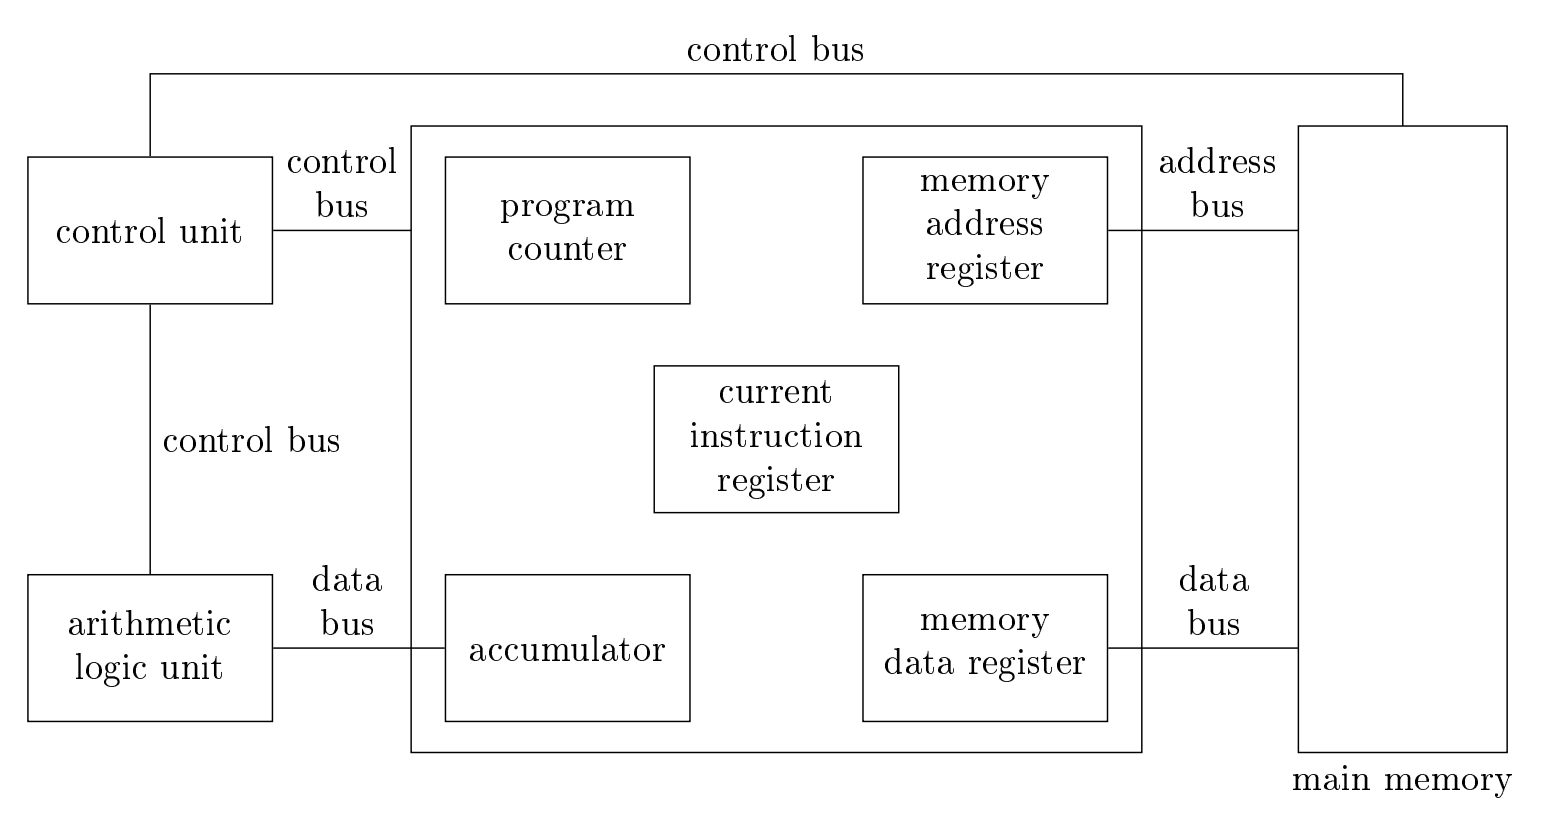
\includegraphics[width=\textwidth]{images/processor-architecture}
	\caption{A simple processor architecture.}
	\label{fig:processor-architecture}
\end{figure}

Figure \ref{fig:processor-architecture} shows the basic schematic of a central
processing unit (CPU). \emph{Buses} are wires that transfer data (or power)
from one location to another. It can link different parts of the CPU
or link the CPU to memory/peripherals.
A bus may fall into one of the follow categories: \emph{data}, \emph{address},
\emph{control}, and \emph{power}.
Furthermore, the method of data transfer can be catergorised:
\begin{enumerate}
	\item point-to-point: transfers data from one location to another;
	\item broadcast: transfers data from one location to many other locations;
		and
	\item bus interface bridges: allows communciation between different bus
		systems (e.g. for communuicating with USB).
\end{enumerate}

Recall that the \emph{radix point} is the symbol used in number systems to
separate the integer part of the number from its fractional part.

We will introduce some examples of converting between decimal and binary.

\begin{examples}
	\begin{enumerate}
		\item $110.11_2 = 6.75_{10}$;
		\item $31.365_{10} = 11111.011_2$; and
		\item $0.10\dot1\dot0_2 = \left(\frac23\right)_{10}$.
	\end{enumerate}
\end{examples}

\begin{definition}[Bytes, nibbles, and words]
	A \emph{byte} is a unit of digital information; 8 bits.
	A 4-bit quantity is called a \emph{nibble}.
	A \emph{word} is a natural unit of data used by a given processor design.
	Modern processors have a word size between 8 bits and 64 bits.
	We may use the terms \emph{half word} and \emph{double word}
	to refer to a unit of data that is respectively half size or double size
	of a normal word size.
\end{definition}

We typically prefix hexadecimal numbers with $\mathtt{0x}$, for example
$\mathtt{0x1234} = 1234_{16}$.

The following are examples of converting between hexidecimal, decimal, and
binary.

\begin{examples}
	\begin{enumerate}
		\item $\mathtt{1F8C.C}_{16} = 8076.75_{10}$; and
		\item $\mathtt{2EF9}_{16} = (0010\,1110\,1111\,0101)_2$.
	\end{enumerate}
\end{examples}

Now we introduce some binary arithmetic.

\begin{examples}
	\begin{enumerate}
		\item $0101_2 + 0111_2 = 1100_2 = 12_{10}$.
		\item $1\,1100_2 \times 0\,1110_2 = 1\,1000\,1000$.
	\end{enumerate}
\end{examples}

\begin{definition}[Integer overflow]
	An \emph{integer overflow} occurs when an arithmetic operation attempts to create a numeric value that is outside of the range that can be represented
	by the given number of digits.
\end{definition}

For example, when adding the 4-bit numbers $1000_2$ and $1001_2$ and storing
the result in a 4-bit register will result in an integer overflow.
When such occurs, a flag in the status register will typically be triggered.

Now we review the possible ways of representing negative binary numbers.

\begin{definition}[Signed magnitutde representation]
	The first bit of a binary number represents whether or not the number
	is positive or negative.
\end{definition}

\begin{definition}[Ones' complement]
	The \emph{ones' complement} of a binary number is defined as the value
	obtained by inverting all the bits.
\end{definition}

A ones' completement system (or arithmetic) is a system in which negative
numbers are represented by the inverse of the binary representation of their
corresponding positive values.

\begin{definition}[Two's complement]
	The \emph{two's complement} of a $n$-bit number is defined to be the value
	of which, when added to the original value, makes $2^n$.
\end{definition}

We can obtain the two's complement of a binary number by adding $1$ to
the ones' complement.
Similarly, negative numbers are represented by the two's complement of the
binary representation of their corresponding positive values.
Two's complement is the most common form of representation for negative 
numbers as it makes binary arithmetic simple.

\begin{table}
	\caption{Examples of binary numbers with their ones' complement and
	two's complement values.}
	\centering
	\begin{tabular}{cccc}
		\toprule
		Bits & Unsigned value & Ones' complement & Two's complement \\
		\midrule
		$0111\,1111$ & 127 & 127 & 127 \\
		$1111\,1111$ & 255 & 0 & 0 \\
		$1111\,0101$ & 245 & -10 & -11 \\
		$0100\,1001$ & 73 & 73 & 73 \\
		\bottomrule
	\end{tabular}
\end{table}

\begin{definition}[Biased representation]
	\emph{Biased representation}, also know as \emph{offset binary} or
	\emph{excess-$K$}, uses a prespecified number $K$ as a biasing value.
	A value is represented by the unsigned number which is $K$ greater than the
	intended value.
\end{definition}

The unsigned value of $1111\,0101$ is 245, while the 
excess-128 interpretation is $117$.

Now we introduce \emph{floating-point representation in binary}.

\begin{definition}[Binary floating-point representation]
	A (typical) floating-point representation has three fields:
	\begin{enumerate}
		\item the sign bit $S$;
		\item the exponent bit $e$; and
		\item the mantissa $M$.
	\end{enumerate}
	This will represent the number \[(-1)^S \times M \times 2^e.\]
\end{definition}

Now we have shown the general foundations for floating-point representation,
we will introduce our first representation.

\begin{definition}[Single-precision floating-point representation]
	A single-precision (32-bit) floating-point number has
	\begin{enumerate}
		\item a $1$-bit sign, $0$ is positive and $1$ is negative;
		\item a $8$-bit exponent, this is stored with excess-$127$ 
			such that it can store a value between $-126$ and $127$; and
		\item a $23$-bit mantissa, this is always scaled such that the
			radix point is after the leading $1$ (we do not store this leading
			$1$, we assume it is there).
	\end{enumerate}
	These are stored sequentially.
\end{definition}

\begin{examples}
	\begin{enumerate}
		\item $0011\,1110\,0010\,0000\,0000\,0000\,0000\,0000 
			= 1.25 \times 2^{-3} = 0.15625$; and
		\item $1100\,0001\,0100\,0110\,0000\,0000\,0000\,0000
			= \frac{99}{64} \times 2^3 = 12.365$.
	\end{enumerate}
\end{examples}